%UNIT 16: Introduction to Laplace Transforms
%%%%%%%%%%%%%%%%%%%%%%%%%%%
%%%% Put the following at the top of each .tex file  %
\pagestyle{fancy}
\renewcommand{\theUnit}{Sections 7.2 and 7.3}
\ifthenelse{\isundefined{\UnitPageNumbers}}{}{\setcounter{page}{1}}
\rhead{\theUnit: Introduction to Laplace Transforms}
\lhead{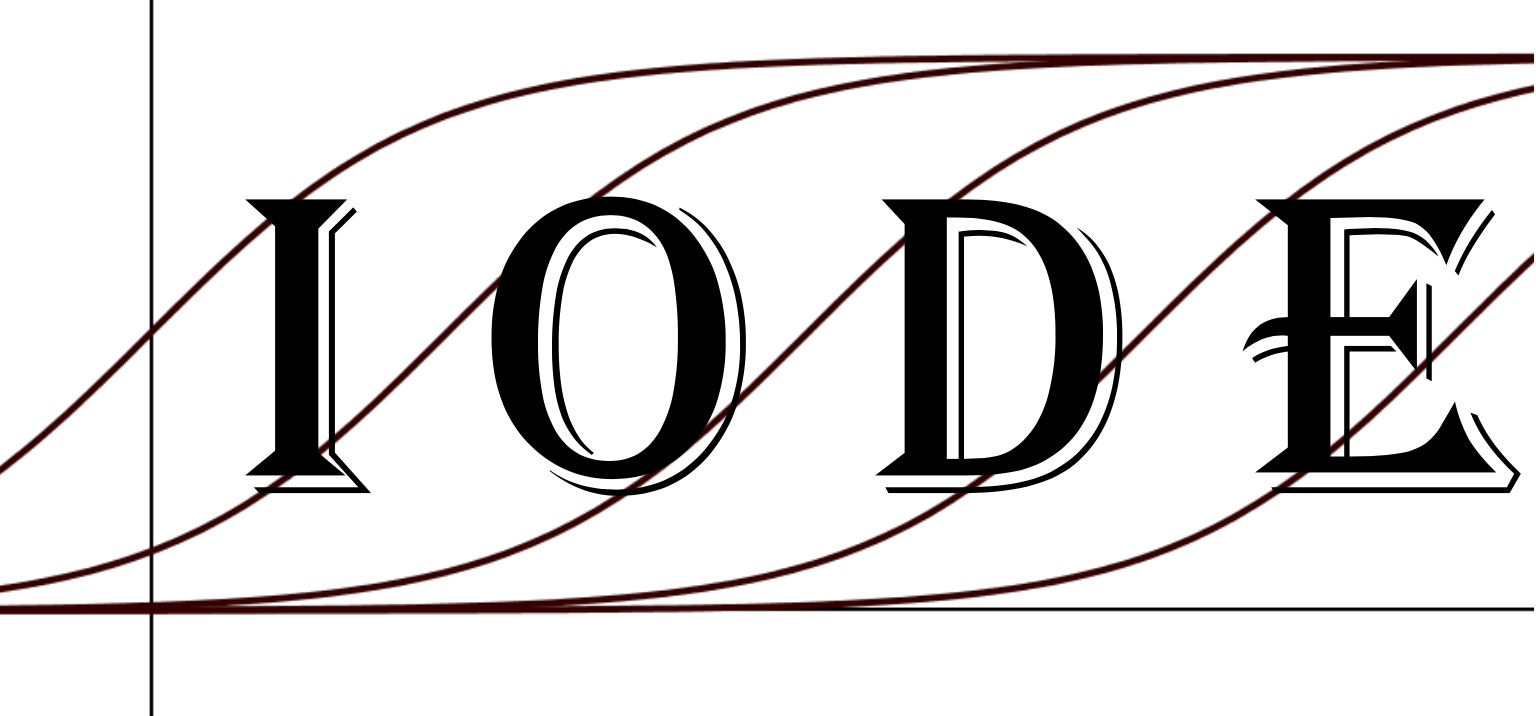
\includegraphics[width=1.25cm]{IODE-logo.png}}
\rfoot{\mypage}
\lfoot{}
\cfoot{}
\fancypagestyle{firstfooter}{\footskip = 50pt}
\renewcommand{\footrulewidth}{.4pt}
%%%%%%%%%%%%%%%%%%%%%%%%%%%
\vspace*{-20pt} \thispagestyle{firstfooter}
\pagebegin{The Laplace Transform}

One of the basic problem solving techniques in mathematics is to 
\bi
\ii transform a difficult problem into an easier one, 
\ii solve the easier problem, and 
\ii then use its solution to obtain a solution of the original problem.
\ei

\bigskip

For example. the reverse product rule (method of integrating factor) is used to transform a linear first order differential equation into an easier problem we can solve. In this chapter we study the method of \textbf{Laplace transforms}, which is one example of this technique. Like the method of integrating factors, Laplace transforms are \textbf{integral operators}. Solving by the method of Laplace transforms:
\bi
\ii Can be used to solve higher order linear differential equations.
\ii Can be applied for more complicated forcing functions.
\ii Requires initial conditions.
%\ii Has applications throughout physics and engineering.
\ei

\bs

The \textbf{improper integral} of $g$ over $\lbrack a , \infty )$ is defined as
\[ \int_a^{\infty} g(t) \ dt = \lim_{N \to \infty} \int_a^N g(t) \ dt.\]
\bi
\ii We say the improper integral \textbf{converges} if the limit exists.
\ii Otherwise we say the improper integral \textbf{diverges}.
\ei


\begin{enumerate}
\ii Determine whether $\dsty \int_0^{\infty} e^{-2t} \ dt$ converges or diverges.
\end{enumerate}

\clearpage

Let $f(t)$ be a function on $\lbrack 0 , \infty )$. The \textbf{Laplace transform} of $f$ is the function $F$ defined by
\[ \Lap \left\{ f \right\} = F(s) = \int_0^{\infty} e^{-st}f(t) \ dt .\]
\bi
\ii The domain of $F(s)$ is all values of $s$ for which the integral converges.
\ii The functions $f$ and $F$ form a \textbf{transform pair}.
\ei


\begin{enumerate}[resume]
  \ii Find and state the domain of the Laplace transform $F(s)=\Lap \left\{ f(t) \right\}$.
  \bb
\ii $f(t) = 2$, $t \geq 0$  \vfill
\ii $f(t) = t$ \vfill 
\ii $f(t) = e^{3t}$ \vfill
%\ii $g(t) = \cos{(bt)}$ where $b \ne 0$ is a constant.
\clearpage

\ii $\dsty f(t) = \left\{ \begin{array}{ll} 
5 \ \ & 0 < t < 2 \\
e^{8t} \ \ & t >2 \end{array} \right.$ \vfill
\ee

%\clearpage



%\clearpage

\bs

\ii Let $f$, $f_1$, and $f_2$ be functions whose Laplace transform exists for $s > \alpha$ and let $c$ be a constant. Then for $s > \alpha$, prove the following:
\bb
\ii $\Lap \left\{ f_1 + f_2 \right\} = \Lap \left\{ f_1 \right\} + \Lap \left\{ f_2 \right\}$. \vfill
\ii $\Lap \left\{ cf \right\} = c \Lap \left\{ f \right\}$. \vfill
\ee
\end{enumerate}

\clearpage

\pagebegin{Properties of the Laplace Transform}

\begin{enumerate}[resume]
\ii If the Laplace transform $\mathscr{L}\{ f \} (s)=F(s)$ exist for $s > \alpha$, then show that
\[ \mathscr{L}\{ e^{at}f(t) \}= F(s-a), \ \ \mbox{for } s > \alpha + a.\]

\vfill

\ii Using the property above and the fact that $\mathscr{L} \{ \cos{(bt)} \} = \frac{s}{s^2+b^2}$ for $s >0$, find
$\Lap \{ e^{at} \cos{(bt)} \}$.

\vfill

\end{enumerate}


A function is of \textbf{exponential order} $\alpha$ if there exists positive constants $C$ and $T$ such that
\[ \left| f(t) \right| < Ce^{\alpha t} \ \ \mbox{for all } t > T.\]
For example:
\bi
\ii $f(t) = \cos{(5t)}e^{7t}$ has $\alpha = 7$.
\ii $e^{t^2}$ does not have an exponential order.
\ei

\begin{enumerate}[resume]
\ii If $f(t)$ is continuous on $\lbrack 0, \infty )$ and $f'(t)$ is piecewise continuous on $\lbrack 0, \infty )$ with
both exponential order $\alpha$, then prove for $s > \alpha$,
\[ \mathscr{L} \{ f' \} = s \mathscr{L}\{ f \} - f(0) = sF(s)-f(0).\]

\vfill

\clearpage

\ii Using the previous problem and the fact that $\mathscr{L} \{ \cos{(bt)} \} = \frac{s}{s^2+b^2}$ for $s >0$, find
$\Lap \{ \sin{(bt)} \}$. \vfill

\ii Using induction show that
\[ \Lap \{ f^{(n)} \} = s^n \Lap \{ f \} - s^{n-1} f(0) - s^{n-2} f'(0) - \ldots - f^{(n-1)}(0).\] \vfill

\ii If $\Lap \{ f(t) \} = F(s)$ for all $s > \alpha$, using the previous problem, show that $\Lap \{ f''(t) \} =s^2F(s)-sf(0)-f'(0)$ for all $s > \alpha$. \vfill
%by induction that $\Lap \{ t^n \} = \frac{n!}{s^{n+1}}$ for $s >0$.

\clearpage

\ii Let $F(s) = \Lap \{ f \}$ and assume $f(t)$ is piecewise continuous on $\lbrack 0, \infty )$ and of exponential order $\alpha$.
Prove that for $s > \alpha$ if follows that
\[ \Lap \{ t^nf(t) \} = (-1)^n \frac{d^nF}{ds^n}.\] \vfill


%\begin{example}
%Show by induction that $\Lap \{ t^n \} = \frac{n!}{s^{n+1}}$ for $s >0$.
\ii Using the definition of the Laplace transform, the result that $\Lap \{ e^{at} \} = \frac{1}{s-a}$ for $s>a$ and the property above, find a formula for  $\Lap \{ t^n e^{at} \}$. \vfill
%\end{example}
\end{enumerate}

\clearpage

\pagebegin{Common Laplace Transforms}

\begin{center}
\begin{tabular}{|l|l|}
\hline
$f(t)$ & $F(s) = \Lap \left\{ f(t) \right\}$ \\
\hline
$1$ & $\dsty \frac{1}{s}, \ s > 0$\\
\hline
$e^{at}$ & $\dsty \frac{1}{s-a}, \ s > a$\\
\hline
$t^n, \ n=1,2, \ldots$ & $\dsty \frac{n!}{s^{n+1}}, \ s > 0$\\
\hline
$\sin{(bt)}$ & $\dsty \frac{b}{s^2+b^2}, \ s > 0$\\
\hline
$\cos{(bt)}$ & $\dsty \frac{s}{s^2+b^2}, \ s > 0$\\
\hline
$e^{at}t^n, \ n=1,2, \ldots$ & $\dsty \frac{n!}{(s-a)^{n+1}}, \ s > 0$\\
\hline
$e^{at}\sin{(bt)}$ & $\dsty \frac{b}{(s-a)^2+b^2}, \ s > a$\\
\hline
$e^{at}\cos{(bt)}$ & $\dsty \frac{s-a}{(s-a)^2+b^2}, \ s > a$\\
\hline
\end{tabular}
\end{center}


%\begin{center}
%\begin{tabular}{|l|l|}
%\hline
%$f(t)$ & $F(s) = \Lap \left\{ f \right\} (s)$ \\
%\hline
%$1$ & $\dsty \frac{1}{s}, \ s > 0$\\
%\hline
%$e^{at}$ & $\dsty \frac{1}{s-a}, \ s > a$\\
%\hline
%$t^n, \ n=1,2, \ldots$ & $\dsty \frac{n!}{s^{n+1}}, \ s > 0$\\
%\hline
%$\sin{(bt)}$ & $\dsty \frac{b}{s^2+b^2}, \ s > 0$\\
%\hline
%$\cos{(bt)}$ & $\dsty \frac{s}{s^2+b^2}, \ s > 0$\\
%\hline
%$e^{at}t^n, \ n=1,2, \ldots$ & $\dsty \frac{n!}{(s-a)^{n+1}}, \ s > 0$\\
%\hline
%$e^{at}\sin{(bt)}$ & $\dsty \frac{b}{(s-a)^2+b^2}, \ s > a$\\
%\hline
%$e^{at}\cos{(bt)}$ & $\dsty \frac{s-a}{(s-a)^2+b^2}, \ s > a$\\
%\hline
%\end{tabular}
%\end{center}


%A function is of \textbf{exponential order} $\alpha$ if there exists positive constants $C$ and $T$ such that
%\[ \left| f(t) \right| < Ce^{\alpha t} \ \ \mbox{for all } t > T.\]

%For example:
%\bi
%\ii $f(t) = \cos{5t}e^{7t}$ has $\alpha = 7$.
%\ii $e^{t^2}$ does not have an exponential order.
%\ei



